\documentclass[12pt]{article}

\usepackage{amsmath}
\usepackage{array}
\usepackage{caption}
\usepackage[top=1in, bottom=1in, left=0.75in, right=0.75in]{geometry}
\usepackage{graphicx}
\usepackage[colorlinks=true, allcolors=blue]{hyperref}
\usepackage[utf8]{inputenc}
\usepackage{multirow}
\usepackage{pdfpages}
\usepackage[section]{placeins}

\graphicspath{{./figures/}}

\begin{document}

\begin{titlepage}
    \begin{center} \LARGE
        \vspace*{1.5in}

        ECE 272 Lab 3

        Fall 2018

        \vfill

        Combinational Logic (Seven-Segment Driver)

        Phi Luu

        \vfill

        October 24\textsuperscript{th}, 2018

        Grading TA: Edgar Perez

        Lab Partner: Benjamin Geyer

        \vspace{1.5in}
    \end{center}
\end{titlepage}

%%%%%%%%%%%%%%%%%%%%%%%%%%%%%%%%%%%%%%%%%%%%%%%%%%%%%%%%%%%%%%%%%%%%%%%%%%%%%%%%
% Introduction
%%%%%%%%%%%%%%%%%%%%%%%%%%%%%%%%%%%%%%%%%%%%%%%%%%%%%%%%%%%%%%%%%%%%%%%%%%%%%%%%
\section{Introduction}

\begin{figure}[h]
    \centering
    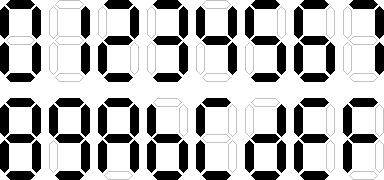
\includegraphics[width=0.5\textwidth]{seven_segment_hexadecimal.png}
    \caption{Seven-segment display showing hexadecimal digits \cite{EEStackExchangeSevenSegmentHex}}
    \label{figure:1}
\end{figure}

%%%%%%%%%%%%%%%%%%%%%%%%%%%%%%%%%%%%%%%%%%%%%%%%%%%%%%%%%%%%%%%%%%%%%%%%%%%%%%%%
% Design
%%%%%%%%%%%%%%%%%%%%%%%%%%%%%%%%%%%%%%%%%%%%%%%%%%%%%%%%%%%%%%%%%%%%%%%%%%%%%%%%
\section{Design}

\begin{figure}[h]
    \centering
    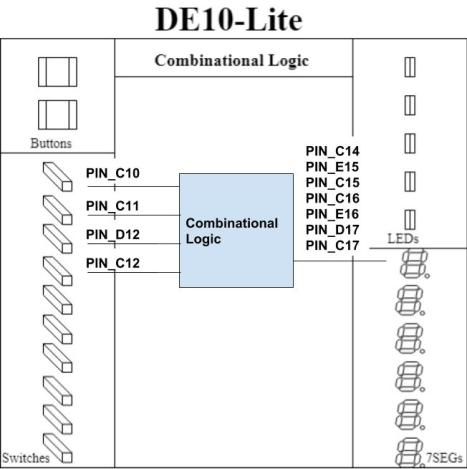
\includegraphics[width=0.5\textwidth]{lab3_block_diagram.png}
    \caption{Block diagram}
    \label{figure:2}
\end{figure}

\begin{table}[h]
    \centering
    \begin{tabular}{ | c | c | c | c | c | c | c | c | c | }
    \hline \rule{0em}{1.15em}
    \textbf{\begin{tabular}[c]{@{}c@{}}Input\\ (Hexadecimal)\end{tabular}} & \textbf{\begin{tabular}[c]{@{}c@{}}Input\\ (4-bit Binary)\end{tabular}} & \textbf{Seg\textsubscript{A}} & \textbf{Seg\textsubscript{B}} & \textbf{Seg\textsubscript{C}} & \textbf{Seg\textsubscript{D}} & \textbf{Seg\textsubscript{E}} & \textbf{Seg\textsubscript{F}} & \textbf{Seg\textsubscript{G}} \\ \hline \rule{0em}{1.15em}
    0                                                                      & 0000                                                                    & 0                             & 0                             & 0                             & 0                             & 0                             & 0                             & 1                             \\ \hline \rule{0em}{1.15em}
    1                                                                      & 0001                                                                    & 1                             & 0                             & 0                             & 1                             & 1                             & 1                             & 1                             \\ \hline \rule{0em}{1.15em}
    2                                                                      & 0010                                                                    & 0                             & 0                             & 1                             & 0                             & 0                             & 1                             & 0                             \\ \hline \rule{0em}{1.15em}
    3                                                                      & 0011                                                                    & 0                             & 0                             & 0                             & 0                             & 1                             & 1                             & 0                             \\ \hline \rule{0em}{1.15em}
    4                                                                      & 0100                                                                    & 1                             & 0                             & 0                             & 1                             & 1                             & 0                             & 0                             \\ \hline \rule{0em}{1.15em}
    5                                                                      & 0101                                                                    & 0                             & 1                             & 0                             & 0                             & 1                             & 0                             & 0                             \\ \hline \rule{0em}{1.15em}
    6                                                                      & 0110                                                                    & 0                             & 1                             & 0                             & 0                             & 0                             & 0                             & 0                             \\ \hline \rule{0em}{1.15em}
    7                                                                      & 0111                                                                    & 0                             & 0                             & 0                             & 1                             & 1                             & 1                             & 1                             \\ \hline \rule{0em}{1.15em}
    8                                                                      & 1000                                                                    & 0                             & 0                             & 0                             & 0                             & 0                             & 0                             & 0                             \\ \hline \rule{0em}{1.15em}
    9                                                                      & 1001                                                                    & 0                             & 0                             & 0                             & 0                             & 1                             & 0                             & 0                             \\ \hline \rule{0em}{1.15em}
    a                                                                      & 1010                                                                    & 0                             & 0                             & 0                             & 1                             & 0                             & 0                             & 0                             \\ \hline \rule{0em}{1.15em}
    b                                                                      & 1011                                                                    & 1                             & 1                             & 0                             & 0                             & 0                             & 0                             & 0                             \\ \hline \rule{0em}{1.15em}
    c                                                                      & 1100                                                                    & 0                             & 1                             & 1                             & 0                             & 0                             & 0                             & 1                             \\ \hline \rule{0em}{1.15em}
    d                                                                      & 1101                                                                    & 1                             & 0                             & 0                             & 0                             & 0                             & 1                             & 0                             \\ \hline \rule{0em}{1.15em}
    e                                                                      & 1110                                                                    & 0                             & 1                             & 1                             & 0                             & 0                             & 0                             & 0                             \\ \hline \rule{0em}{1.15em}
    f                                                                      & 1111                                                                    & 0                             & 1                             & 1                             & 1                             & 0                             & 0                             & 0                             \\ \hline
    \end{tabular}
    \caption{Conversion table between hexadecimal, 4-bit binary, and seven-segment decoder}
    \label{table:1}
\end{table}

\begin{figure}[h]
    \centering
    \includegraphics[width=\textwidth]{lab3_schematic.png}
    \caption{A schematic for the seven-segment display decoder. Due to the large difference between the size of the schematic and the available space, an image with higher resolution has been uploaded \href{https://i.imgur.com/jaLoZg9.jpg}{here}.}
    \label{figure:3}
\end{figure}

\begin{figure}[h]
    \centering
    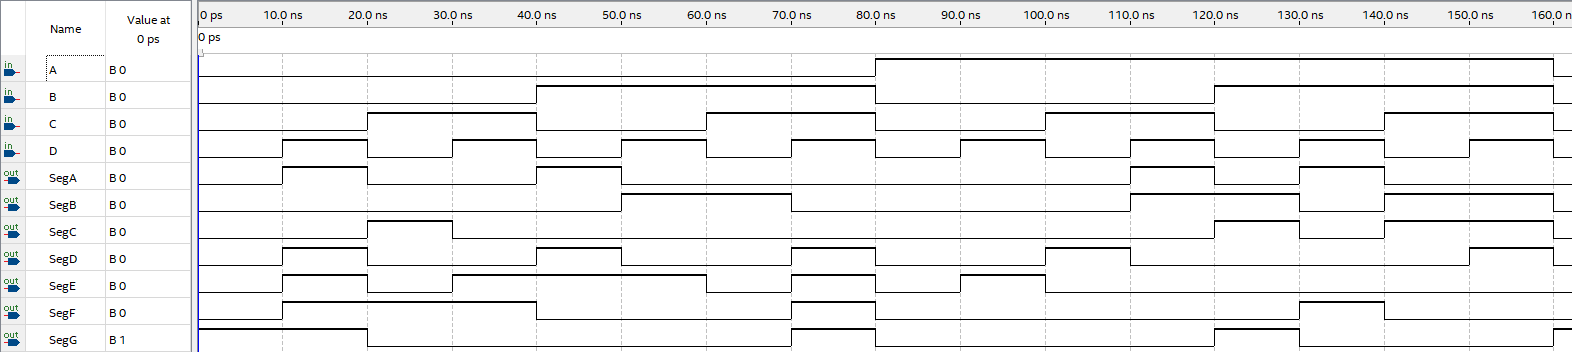
\includegraphics[width=\textwidth]{lab3_simulation.png}
    \caption{Simulation waveform of the program with each 10-nanosecond interval representing a hexadecimal digit}
    \label{figure:4}
\end{figure}

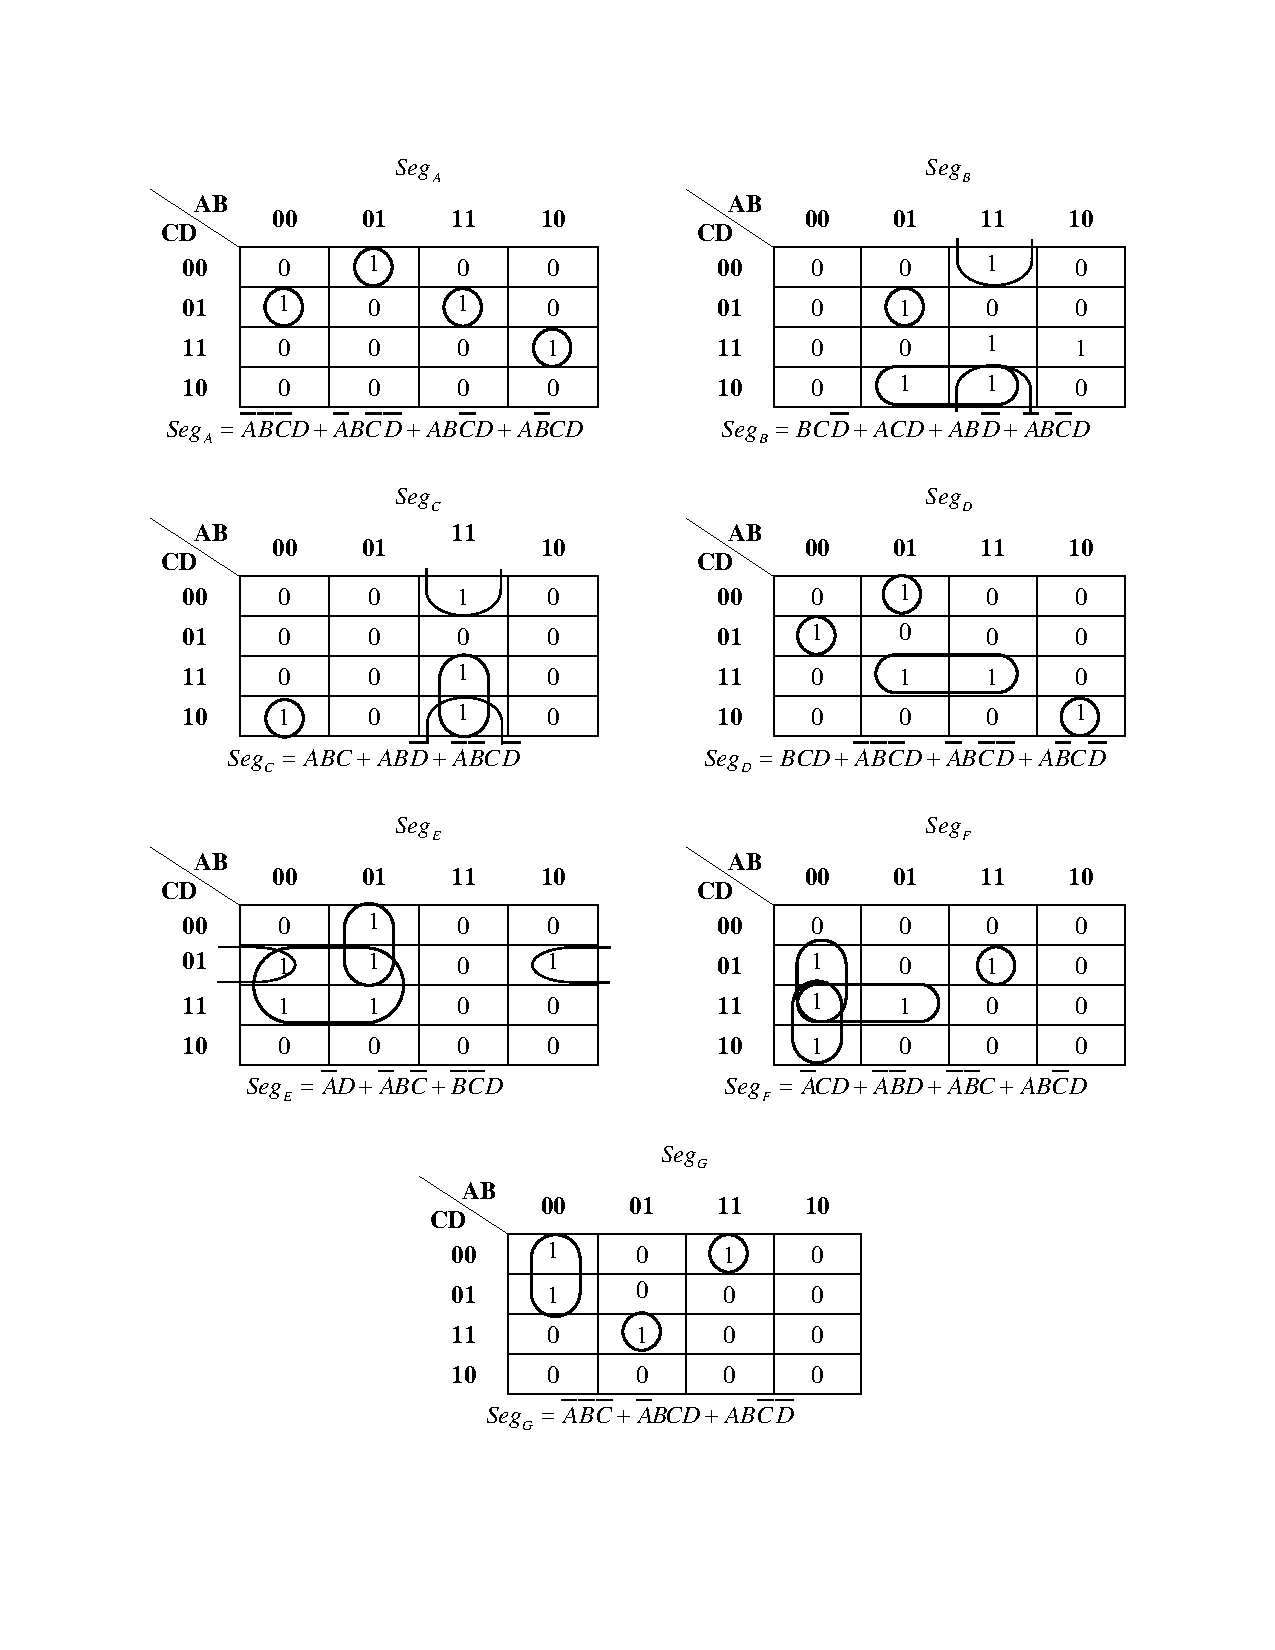
\includepdf[page=-]{lab3_karnaugh_maps}

%%%%%%%%%%%%%%%%%%%%%%%%%%%%%%%%%%%%%%%%%%%%%%%%%%%%%%%%%%%%%%%%%%%%%%%%%%%%%%%%
% Results
%%%%%%%%%%%%%%%%%%%%%%%%%%%%%%%%%%%%%%%%%%%%%%%%%%%%%%%%%%%%%%%%%%%%%%%%%%%%%%%%
\section{Results}

%%%%%%%%%%%%%%%%%%%%%%%%%%%%%%%%%%%%%%%%%%%%%%%%%%%%%%%%%%%%%%%%%%%%%%%%%%%%%%%%
% Experiment Notes
%%%%%%%%%%%%%%%%%%%%%%%%%%%%%%%%%%%%%%%%%%%%%%%%%%%%%%%%%%%%%%%%%%%%%%%%%%%%%%%%
\section{Experiment Notes}

%%%%%%%%%%%%%%%%%%%%%%%%%%%%%%%%%%%%%%%%
% Reflection
%%%%%%%%%%%%%%%%%%%%%%%%%%%%%%%%%%%%%%%%
\subsection*{Reflection}

%%%%%%%%%%%%%%%%%%%%%%%%%%%%%%%%%%%%%%%%
% Study Questions
%%%%%%%%%%%%%%%%%%%%%%%%%%%%%%%%%%%%%%%%
\subsection*{Study Questions}

\begin{enumerate}
    \item When is a simulation necessary? Was it useful for this section?
\end{enumerate}

%%%%%%%%%%%%%%%%%%%%%%%%%%%%%%%%%%%%%%%%%%%%%%%%%%%%%%%%%%%%%%%%%%%%%%%%%%%%%%%%
% Appendix
%%%%%%%%%%%%%%%%%%%%%%%%%%%%%%%%%%%%%%%%%%%%%%%%%%%%%%%%%%%%%%%%%%%%%%%%%%%%%%%%
\section*{Appendix}

No appendix is available in this lab.

%%%%%%%%%%%%%%%%%%%%%%%%%%%%%%%%%%%%%%%%%%%%%%%%%%%%%%%%%%%%%%%%%%%%%%%%%%%%%%%%
% Bibliography
%%%%%%%%%%%%%%%%%%%%%%%%%%%%%%%%%%%%%%%%%%%%%%%%%%%%%%%%%%%%%%%%%%%%%%%%%%%%%%%%
\bibliographystyle{ieeetr}
\bibliography{references}

\end{document}
